\documentclass{article}
\usepackage{graphicx}
\usepackage{enumitem}
\usepackage{pdfpages}
\usepackage{multicol}
\usepackage[a4paper, left=1in, right=1in, top=1in, bottom=1in]{geometry}
\usepackage[ngerman]{babel}
\usepackage{fancyhdr}
\pagestyle{fancy}

% Header
\fancyhead[L]{Niklas Fister}
\fancyhead[C]{Kantonnschule Wettingen - Deutsch}
\fancyhead[R]{\thepage}

% clear Footer
\fancyfoot{}

% Title
\title{\huge\textbf{Gegenwartsliteratur}}
\author{Niklas Fister}
\date{\today}

\begin{document}
\maketitle
\newpage

\section{Epochen}

\subsection{Einführung}
\begin{itemize}[parsep=0pt]
    \item Keine Eoche, sondern alles was in der aktuellen Zeit entstand - Es handelt sich somit um eine Rahmenbedinung
    \item Grobe Unterteilung ist die Literatur seid dem 2. WK und die genaue seid dem Mauerfall 1989
    \item Die Postmoderne ist teil der Gegenwartsliteratur und ist zwischen 1968 - 200 oder 1989 - 2011. Sie ist sozusagen die Gegebewegung zur Moderne.
    \item Ein Ansatz war von der digitalisierung als Start (1970) auszugehen.
\end{itemize}
\subsubsection{Merkmale}
\begin{itemize}[parsep=0pt]
    \item Es wird eine morderne, einfache Schreibweise verwendet.
    \item Durch die Freiheit der heuteigen Zeit, gibt es keine Regeln und man kann schreiben, wie man will. Somit entstehen unterschiedliche Arte von Werken.
    \item Die Literatur soll zum Denken anregen und nicht die aktuelle Epoche kritisieren.
    \item Die Themen: Globalisierung, Digitalisierung, Kapitalismus, Pluralismus, sowieso Erinnerungsliteratur und der aktuellen Politischen Gesellschaft.
    \item Bei der Globalisierung sind dramatische Vorfälle wie Terroranschläge und Klimawandel ein Thema. Zudem wird die Politik wie zum Beispiel die AfD und andere "Organisationen" thematisiert.
    \item Neue Formen die entstanden sind: Interkulturelle Literatur, Netzliteratur und Regiertheater
\end{itemize}

\section{Buch - Glitsch}
\subsection{Autor - Adam Schwarz}
Der Name ist ein Pseudonym und entstand durch seinen schwarzen Humor. Es entstand durch seine Grossmutter ihren willen im Internet seine Texte zu suchen.

Er ist ein Schweizer Autor und hat in Zürich studiert.
\subsection{Inhalt}
\begin{multicols}{2}
Es handelt sich um eine das Paar Kathrin, was auf einem Kreuzfahrtschiff. Das Schiff wurde von ihren reichen Eltern finanziert und die beide haben Konflikte, da sie ihn gar nicht dabei haben wollte.

Plötzlich verschwindet Kathrin und anschliessend kommt León nicht mehr in sein Zimmer und er ist im System des Schiffes nicht mehr vorzufinden. Er wird verdächtigt illegal auf dem Schiff zu sein und kommt in ein Zimmer mit Willem.

Später enttapte er eine Sekte durch C.C. Salarius, welche er auf dem Schiff in der Nacht fand. Dabei erkannte er Kathrin und Willen, wobei es auch ein Truam sien konnte.

Algen wurden immer mehr ein Zeichen für die Mystik. Am Ende entscheidet sich León zurück auf das Schiff zu gehen, um Kathrin zu retten.
\end{multicols}
\subsection{Themen}
\begin{itemize}[parsep=0pt]
    \item Kreuzfahrt und Umwelt - León kritisiert das schädliche der Kreuzfahrt und die Menschen auf dem Schiff leben nicht umweltbewusst und es wird viel verwschwendt
    \item Bezihung - Die holprige Beziehung zwischen Kathrin und León
    \item Gesellschaft - Die Gesellschaft, welche sich nicht auf andere einlässt und egoistisch handlete.
    \item Gaming - Der Gltisch im Spiel, welch es auch spannend machen
    \item Erlösung - Die Sekte, welche wieder zum Wasser zurückkehren wollen und sich dabei fast ertrenkten.
\end{itemize}

\section{Auftrag}
\subsection{Aufgabe 1}
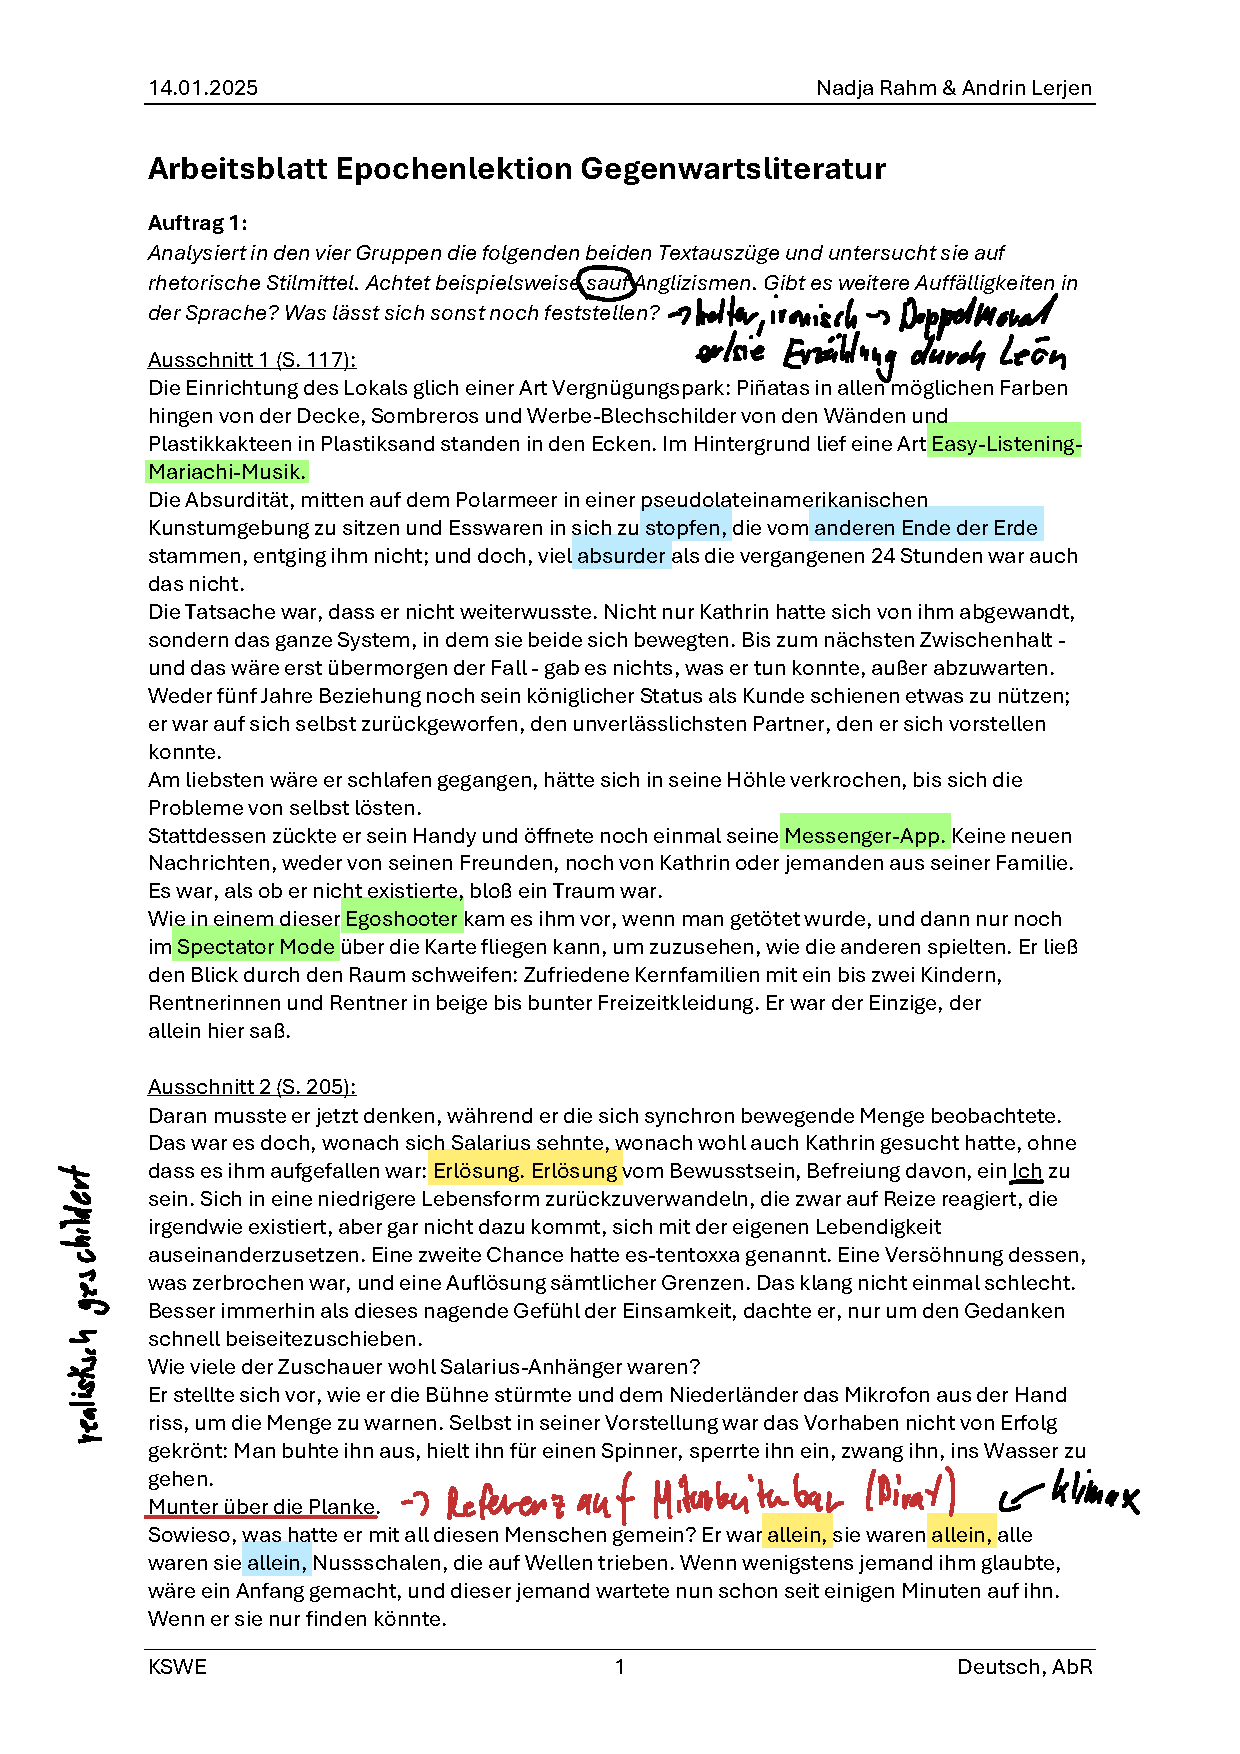
\includepdf[pages=-]{resources/pdfs/Arbeitsauftrag_Buch_Gegenwartsliteratur.pdf}
\subsection{Aufgabe 2}
\textbf{Rechtsrutsch}
\begin{multicols}{2}
\begin{itemize}[parsep=0pt]
    \item Frust: Unzufriedenheit
    \item Verschwörungstheorien
    \item Früher war alles besser
    \item Gefühl abgehängt zu werden / Benachtteiligung /Diskriminierung
    \item Der ständige Vorwurf etwas falsch zu machen
    \item Sehensucht nach einfacher Lösung (durchgebracht durch mangelnde Bildung)
    \item Xenophobie / Ausländer:innen hasse / Traditionelle Röllenblider, welche zurückgerufen werden / Selbstjustiz / Armut
    \item Die Angst vor dem Verlust der eigenen Identität
    \item Erstarkender nationalismus - Globale Probleme werden nur im Inneren diskutiert
    \item Abgrenzung und Isoluierung - fehlender Glaube an die Medien
\end{itemize}
\end{multicols}
\section{Diskussion}
\subsection{Glitsch}
Die heutige Technologie kann unsere Wahrhenmung stark beeinflusen. Seine eigene Meinung wird stark von was wir durch die Algorithmen vorgeschlagen bekommen beeinflusst.

Einerseits kann man sich deutlich besser informieren, andererseits wird oftmals viel verschönert. Es verzieht damit unsere Wahrhenmung (romantisierung).

Durch KI muss man vorsichtig sein, was man glauben kann/darf und was nicht mehr der Realität entspricht.

In der heutigen Zeit ist es wichtig selbst über seine Handlungen zu reklektieren und seine Fehler einzusehen, aber auch klar von dem abgrenzen, für was man nichts kann.

Bei Sachen wie einer Klimakriese muss die ganze Gesellschaft zusammenarbeiten. Vor allem die Hauptverursacher müssen handln.

Es ist eine Verantwortung sich seiner Macht bewusst sein.

\subsection{Eoche}

In 2050 wird man vermutlich über die radikalisierung der aktuellen Politik diskutieren. Die Wahlen der USA und en allgemeinnen Rechtsrutsch werden Thema sien.

Die Entwicklungen der KI und die somit resultierende Änderungen in Gesellschaft und Wirtschaft werden essentiell sein.

\end{document}